\section{Introduction}
\label{sec:intro}
%
%Outline of the introduction:
%
%\begin{itemize}
%\item What is ``free association''?
%\item What is semantic similarity: taxonomic similarity vs. relatedness,
%and the common approches to compute these, i.e.,
%either by a knowledge base or corpus based (LSA).
%\item Why is free association more suitable for computing semantic similarity?
%One thing we might argue is that it supports both types of similarity?
%\item However the existing free association network is limited in scale -
%can't support semantic similarity well, even though in theory it is promising.
%\item We expand the current free association network using 6 types of
%co-occurrence information from Wikipedia corpus. The network
%contains disambiguated concepts and is also scalable.
%\item This network supports the computation of term similarty as well as
%short text similarity.
%\item Our contributions: (1) Empirically showed that free associaton is a
%competent alternative knowledge base for computing semantic
%similarity/relatedness; (2) Build a large scale ``synthetic'' free association
%network from Wikipedia; (3) Demonstrated that this network can be used to
%effectively compute both term similarity and short text similarity and
%achieve state-of-the-art accuracies.
%\end{itemize}
%
Computing semantic relatedness between two words (or texts)
is a fundamental task in natural language processing,
artificial intelligence and information retrieval. Strictly
speaking, semantic relatedness is a more general notion than
semantic similarity as it captures not only closeness between two
objects within a type hierarchy (e.g., river and stream), but also
any other relations (e.g., river and boat) \cite{Budanitsky:2006}.
Traditionally, semantic similarity has been computed either within
some lexicon \cite{Roget_Jarmasz,Resnik:1995,Jiang:1997,Lin:1998} 
or by comparing the distributional properties
of contexts \cite{LSA,ESA,SSA}.  On the
other hand, semantic relatedness has been largely modeled by
co-occurrences within a window in a large text corpus.

For both similarity and relatedness, co-occurrences play a central
role, hence how they are extracted and combined can significantly
influence the quality of relatedness computation. 
%For example,
%although web pages are probably the largest source of text data on
%earth, they contain excessive noise which makes co-occurrence
%information less reliable. 
So far, dozens of similarity functions
\cite{mcgill1979evaluation} 
have been proposed for IR, all of which involving co-occurrences in
one way or another, but few achieve satisfactory results on both
similarity and relatedness. The reason for such limited success, we
argue, is that, since similarity and relatedness are ultimately
human perceptions and thus evaluated against human annotated scores,
simple window-based co-occurrences, often contaminated with noises, offer insufficient signals to
match the human perception. In other words, there exists a
perceptional gap between the relatedness perceived by humans and the
co-occurrences we collect from text corpora.

As a human perception signal to bridge such gap, we consider a
well-studied psychological process called {\em free association}. In
free association, a person is given a {\em cue} word and is asked to
produce the first word that comes to her mind as the {\em response}. Previously, a number
of free association experiments by psychologists
resulted in a few data sets called {\em free association norms}.
\tabref{tab:florida} is a fragment of the free association norms collected by
University of South Florida \cite{Nelson:2004}, known as Florida
Norms from now on.

\begin{table}[ht]
\begin{center}
\caption{The strongest reponses to the cue word ``river''}
\begin{tabular}{lrr}\hline
Cue &   Response    &Strength \\\hline
river&    lake&       15/150 \\
river&    stream&      15/150\\
river&    water&      9/150\\
river&    flow&    8/150\\
river&    boat&       7/150\\
river&    canoe&        7/150\\
\hline
\end{tabular}
\end{center}
\label{tab:florida}
\end{table}

Each row of the data contains a cue word, a response word and the
strength of the association (a fraction of the people who
responded with this pair of association in the experiment). 
The free association norms can be viewed as a network in which 
nodes are the words, and edges carry the strengths.
One can see that edges in this network connect both similar pairs
(e.g., river and stream) and related ones (e.g., river and boat), which
seems ideal for computing semantic relatedness. However, this network suffers from two limitations. First, the
number of cue words in these datasets ranges from 100 to 5000, 
which means only the most
common English words are covered and the scale of such a network is
too small for predicting the relatedness score between two arbitrary
words. Second, due to the cost of free association experiments, the
number of human subjects is usually small. A cue word is 
typically presented to a few dozens to 1000 subjects, yielding a few dozens
unique responses. 
Thus the free association network is fairly sparse.
%This is evident in the above example as well, where the association
%between river and flow is stronger than river and boat.

In this paper, we propose a novel approach to construct a large-scale,
comprehensive association network of English terms and concepts by
combining semantic signals
from both free association norms and Wikipedia.
Wikipedia is a large, high-quality text corpus from which
co-occurrences can be drawn. In the past, people primarily extracted
co-occurrences between terms within the Wikipedia article body.
%These approaches have ignored the rich structure and extensive meta
%data within Wikipedia.
%As such, even though Wikipedia-related approaches
%produced state-of-the-art results in modeling semantic relateness,
%there is still a substantial room for improvement when it comes to
%correlation with the human labels.
Instead, we leverage the rich structure within Wikpedia, to
%In contrast, we leverage structures to 
extract 5 types of co-occurrences, which are then
aggregated into a single, universal association strength score by
learning from the strengths of the free association norms. Such
scores are used to weight the edges in the proposed association
network. This network can be thought of as an expanded, smoothed
version of the free associate network, and can be used to simulate how
an average human being associates one concept to another in her
mind. We would then use this association network to compute the
semantic relatedness between terms and short texts.\footnote{In this paper,
we use ``short text relatedness'' and ``short text similarity'' interchangeably.}
%Each node of this network is an English word or
%term; each directed edge carries the strength of association from one
%word to another.

In summary, this paper makes three main contributions.
\begin{enumerate}
\item We extract 5 different types of co-occurrences
from Wikipedia and construct a ``synthetic''
association network by training on free association norms (\secref{sec:approach});
%\item We propose methods to compute term-to-term relatedness and
%short text similarity using this network;
\item We empirically show that free association is a
competent alternative source of knowledge for computing semantic
relatedness, and our ``synthetic'' association network 
effectively simulates free association and resolves its limitations (\secref{sec:free} and 
\secref{sec:predict});
\item We propose algorithms to compute semantic relatedness based on the constructed association network
, which outperform state-of-the-art methods
(\secref{sec:term}).
\end{enumerate}

%The rest of the paper is organized as follows.
%\secref{sec:approach} will describe the data sources we used,
%and present a basic algorithm and an advanced algorithm to construct
%the association network, and how to calculate relatedness using this network.
%\secref{sec:eval} shows how this technology is useful in similarity
%computation task. Finally we compare our work with
%a large body of related work in \secref{sec:related} and conclude the paper
%in \secref{sec:conclude}.
%How humans associate one concept with another is a fundamental topic in
%cognitive science. And how to model this process in computer systems with given data and use it to solve practical problems is an essential issue in cognitive computing.
%With better understanding and modelling of the mental association process we call ``mind-drifting'',
%we can provide better solutions to various problems like relatedness computing, which is
%an essential problem in data mining and natural language processing (NLP),
%as relatedness is frequently used in many applications
%such as information retrieval, recommendation systems, question answering
%and human computer interaction.
%
%\subsection{Research Background}
%To model the concept association process in human brains, there is much existing work in Free Association field, a technique first used in psychoanalysis (and also in psychodynamic theory) which was originally devised by Sigmund Freud. And it was considered as the first instrument for the scientific examination of the human mind \cite{freud1977sexuality}.
%In today's free association experiments, participants are typically required to produce the first word to come to mind that is related in a specified way to a presented cue \cite{Nelson:2000}. Using this experiment method, several free association datasets were built, which can be used to help us understand several kinds of important mental process such as comprehension, elaboration, retrieval \cite{jenkins1979four} as well as many key issues in memory, priming, language, reason and development \cite{Nelson:2004}. Besides, they are also used to evaluate statistical models of semantic representation \cite{gillund1984retrieval} \cite{Dennis:2003} and determine whether some specialized population deviates from the norm \cite{reich2005exploring}. In the construction of our concept association network, we resort to a gold standard dataset in Free Association field to make our network reflect human's association process.
%
%Traditionally, relatedness has been explored in the context of
%semantic {\em similarity}. Strictly speaking, there are two types
%of similarity. One measures the degree of {\em commonality}
%between two objects, e.g., football and soccer;
%the other one estimates the degree of {\em relatedness}
%between two objects, e.g., soccer and World Cup. The first type of similarity
%is usually computed with the help of a taxonomy system such as WordNet
%\cite{Resnik:1995} \cite{Jiang:1997} \cite{Lin:1998} or Probase \cite{LiPeipei:2013}.
%The second type is commonly referred to as relatedness, and on the other hand, it has been
%computed from distributional properties from large text corpora
%\cite{Strube:2006} \cite{Chen:2006} \cite{Gabrilovich:2007} \cite{Bollegala:2011}.
%Some of the corpora used include web text \cite{LiPeipei:2013}, search engine snippets
%\cite{Sahami:2006} and Wikipedia articles \cite{Gabrilovich:2007}.
%The primary feature used in all these systems is
%{\em term-term co-occurrence} information. That is, two terms
%are considered related, {\em if and only if} they co-occur frequently
%within a window in a document. Such window can be a sentence, a paragraph,
%or a document. Because the above definition of relatedness relies heavily on
%the number of co-occurrences, it does not work very well when the
%corpus is not large enough and thus the sample of co-occurrence
%doesn't correspond to the real distribution.
%In other words, previous work merely attempts to derive
%the strength of direct connection between two concepts, ignoring the fact
%that two concepts might be connected not through direct co-occurrence, but
%only through a number of other {\em latent} concepts.
%And this process we call {\em mind drifting}, will be the focus of
%our discussion in this paper.
%
%\subsection{Definition and Description}
% This paper proposes a new idea to model what we would like to call ¡°mind-drifting¡±, the real association process happening in one¡¯s mind when he or she tries to understand natural language (for example a question) and recall related knowledge. In mind-drifting process, for any specified term pair A and B, we try to measure the probability one can associate A with B or vice versa, and the latent path through which such association is achieved. And we base our algorithm on two points, that is concepts may be connected not directly but through several latent bridge concepts to form a mind-drifting chain, and that each step of the mind-drifting process happens under a certain context and the association process can be different under different context. Then we can build a concept association network from datasets in any language based on the model, and discover mind-drifting chain and compute semantic relatedness more precisely. Finally we aim to apply our model to various applications like recommendation systems, information retrieval systems and question answering systems.
%
%%\begin{figure}[th]
%%\centering
%%\epsfig{file=network.eps,width=\columnwidth}
%%\caption{A Fragment of the Concept Association Network}
%%\label{fig:can}
%%\shrink
%%\end{figure}
%
%Our inspiration comes from the association activity in real human brain.
%In human mind, the direct association from one concept to another is
%limited to relatively strong connections,
%while for relatively weak connections, human would probably complete
%the association by ``drifting'' through other bridging concepts, where each
%such bridge is a strong enough connection.
%
%For example, when we mention the concept ``football'',
%one probably has little chance of being reminded of the pop group
%``Spice Girls'', for they don't have much
%in common, nor do they appear together frequently in any context.
%However, it is very likely and quite natural for people to drift their mind
%from ``football'' to ``David Beckham'', the world-renown British footballer,
%then from ``David Beckham'' to his wife
%``Victoria Beckham", and finally from ``Victoria Beckham''
%to her former pop group ``Spice Girls''. This path of connection allows us
%to associate seemingly remote concepts together in a concept association
%network, which we call {\em MindDrifter} in this paper.
%
%Looking into the mind drifting process,
%we discover two important characteristics:
%First, each step of the association is only affected by
%the previous step, that is, the associate process is typically
%a one-way chain. Second, each step of association happens under
%certain context.
%For example, at the mention of ``David Beckham'', Spanish sports fans
%may first think of ``Real Madrid'' and the days David spent there;
%while fashion and music lovers may first think of ``Victoria Beckham''
%and latest news about the couple. With these two typical features,
%one natural solution to model the mind drifting process is HMM
%(Hidden Markov Model) \cite{rabiner1986introduction}. That is, each state in the HMM model is the
%probability distribution of every possible contexts.
%And under each certain state, the observable result will be the probability of thinking of concept B at the mention of concept A under this state.
%Then we can model the mind drifting process and use it to calculate the relatedness between concepts in human mind.
%
